\chapter{Reglementen \& Voorrangsregels}
\vspace{-120px}
\section*{Wie heeft er voorrang? Denk ook goed na waarom en vul de letter in!}
\begin{table}[h!]
\centering
\begin{tabular}{l|l|l|l|l|l|l|l|l|l|l|l|l|l|l}
\textbf{1} & \textbf{2} & \textbf{3} & \textbf{4} & \textbf{5} & \textbf{6} & \textbf{7} & \textbf{8} & \textbf{9} & \textbf{10} & \textbf{11} & \textbf{12} & \textbf{13} & \textbf{14} & \textbf{15} \\ \hline
 \hspace{0.5 cm} & \hspace{0.5 cm}  & \hspace{0.5 cm} & \hspace{0.5 cm} & \hspace{0.5 cm} & \hspace{0.5 cm} & \hspace{0.5 cm} & \hspace{0.5 cm} & \hspace{0.5 cm} & \hspace{0.5 cm} & \hspace{0.5 cm} & \hspace{0.5 cm} & \hspace{0.5 cm} & \hspace{0.5 cm}
\end{tabular}
\end{table}
\begin{figure}[h!]
    \centering
    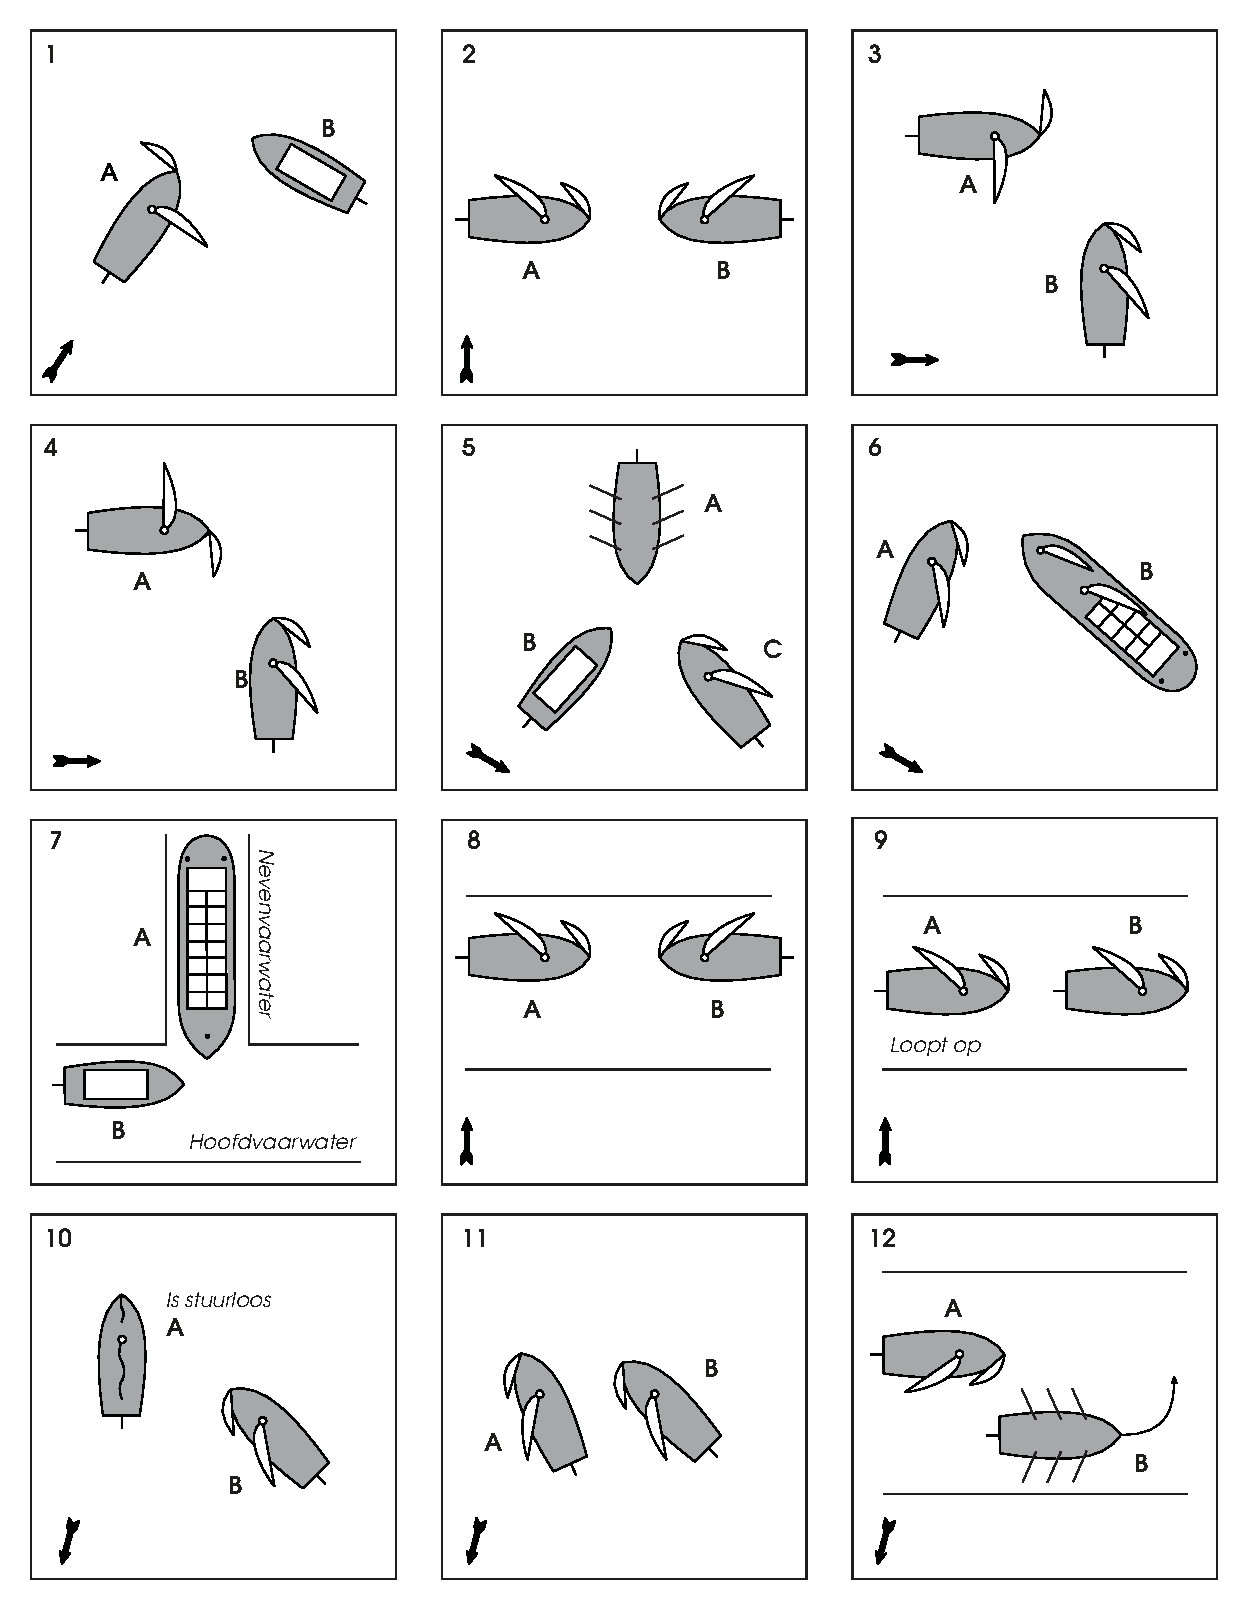
\includegraphics[width=\textwidth]{Hoofdstukken/Oefenvragen/pdf/regelementen_1.pdf}
\end{figure}

\newpage
\begin{figure}[h!]
    \centering
    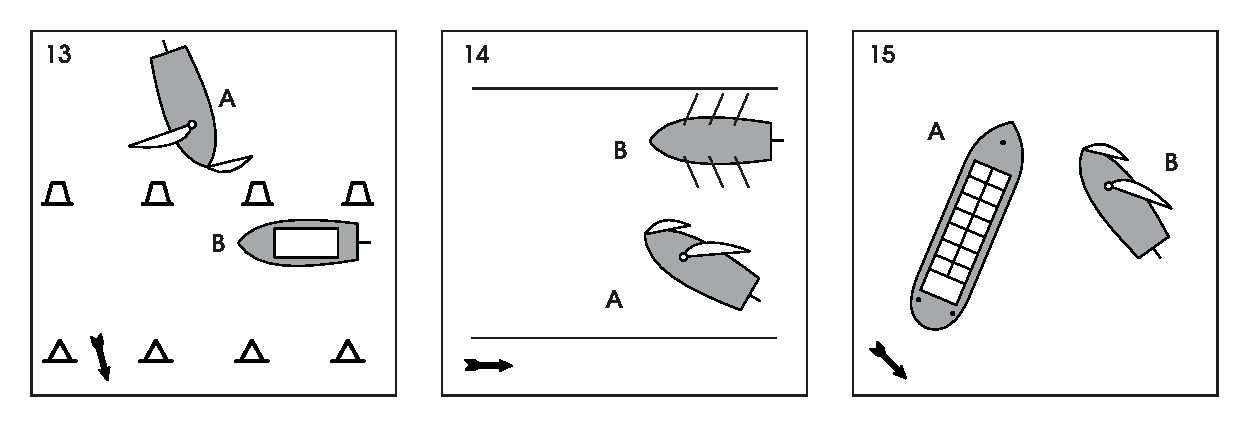
\includegraphics[width=\textwidth]{Hoofdstukken/Oefenvragen/pdf/regelementen_2.pdf}
\end{figure}
Bij sommige van de vorige situaties is een extra vraag. Het vraagnummer van de onderstaande vragen geeft aan naar welk figuur je moet kijken.\vspace{2cm}

\question{5}{Op welke volgorde mogen de boten verder varen?}
\answerTextFour{A-B-C}{C-B-A}{C-A-B}{B-C-A}

\question{9}{Welke koersen varen de schepen ten opzichte van elkaar?}
\answerTextFour{Kruisende koers}{Voorbijlopende koers}{Oplopende koers}{Tegengestelde koers}

\question{10}{Welke stelling is waar?}
\answerTextFour{B heeft voorrang want hij heeft zijn zeilen over bakboord}{A heeft voorrang, je kan namelijk niet zien over welke boeg zijn zeilen staan}{A heeft voorrang, hij vaart lij}{B moet uitwijken. A is stuurloos, er ontbreken regels dus goed zeemanschap geldt}

\question{12}{Wie heeft er voorrang en waarom?}
\answerTextFour{A, want zeil gaat voor spier gaat voor motor}{A, want B steekt een vaarwater over}{B, want hij vaart stuurboordwal}{B, want hij is aan het manoeuvreren}

\question{13}{Wie heeft er voorrang en waarom?}
\answerTextFour{A, want zeil gaat voor spier gaat voor motor}{B, want A steekt een vaarwater over}{B, want hij vaart stuurboordwal}{B, want A komt van links}